\documentclass[a4paper,12pt]{article}

\usepackage[document]{ragged2e}
\usepackage[portuguese]{babel}
\usepackage[utf8]{inputenc}
\usepackage[numbers]{natbib}
\usepackage{multirow}
\usepackage{booktabs}
\usepackage[a4paper, left=3cm, right=2cm, top=3cm, bottom=2cm]{geometry}
\usepackage{multicol}
\usepackage{multirow}
\usepackage{graphicx}
\graphicspath{{./Imagens/}{../image/}}
\usepackage{times}
\usepackage{amssymb,amsmath}
\usepackage[binary-units=true]{siunitx}
\usepackage{bbm}
\usepackage{color}
\usepackage[active]{srcltx}
\usepackage{url}
\usepackage{float}
\usepackage{setspace}
\usepackage{colortbl}
\usepackage{units}
\usepackage{tikz}
\usepackage{verbatim}
\usetikzlibrary{shapes.arrows}
\usepackage{multirow}
\usepackage{fancyhdr}
\usepackage{scalefnt}
\usepackage{helvet}
\usepackage{indentfirst}
\usepackage{parskip}
\usepackage{subcaption}


\begin{document}
    \begin{center}
        \includegraphics[width=.30\linewidth]{logo.png}
    
        \textbf{UNIVERSIDADE FEDERAL DE ALAGOAS}
    
        \textbf{PRÓ-REITORIA DE PÓS-GRADUAÇÃO E PESQUISA}
    
        \textbf{NÚCLEO DE INOVAÇÃO TECNOLÓGICA}
    
        \textbf{PROGRAMA INSTITUCIONAL DE BOLSAS DE INICIAÇÃO EM
        DESENVOLVIMENTO TECNOLÓGICO E INOVAÇÃO}
    
        \textbf{PIBITI 2018-2019}
    
        \textbf{RELATÓRIO FINAL}
    \end{center}
    
    \begin{table}[h]
        \centering
        \begin{tabular}{|p{7,5cm}|p{7,5cm}|} \hline 
             \textbf{Título do projeto de pesquisa: }& Software científico para análise e processamento de imagens PolSAR \\ 
             \hline
             \textbf{Orientador: }& Alejandro César Frery Orgambide  \\  
             \hline
             \textbf{Título do plano de trabalho individual:} & Desenvolvimento do software com as funcionalidades criadas para processamento, análise e visualização de imagens SAR/polSAR. \\ 
             \hline
             \textbf{Discente:} & Ulilé Indeque\\ 
             \hline
             \end{tabular}
             \begin{tabular}{|p{15,45cm}|}
             \textbf{Cota: (X)CNPQ ( )UFAL ( )FAPEAL ( )COLABORADOR} \\ 
             \hline
        \end{tabular}
        \begin{tabular}{|p{7,5cm}|p{7,5cm}|}
            \textbf{Demais envolvidos (Instituições, pesquisadores, empresas):} & \\ \hline
             \textbf{Unidade acadêmica:} &  IC\\
            \hline
            \textbf{Local de execução (Laboratório):} &  Laboratório de Computação Científica e Análise Numérica\\
            \hline
            \textbf{Fontes de financiamento:} & \\ 
            \hline
            \textbf{Grande área do conhecimento (CNPq):} &  Ciências Exatas e da Terra\\
            \hline
            \textbf{Área do conhecimento (CNPq):} &  Ciência da Computação\\
            \hline
            \textbf{Sub-área do conhecimento (CNPq):} &  Sistemas de Computação\\
            \hline
            \textbf{Especialidade do conhecimento (CNPq):} &  Processamento Gráfico (graphics)\\
            \hline
        \end{tabular}
        \begin{tabular}{|p{3,05cm}|p{3cm}|p{5cm}|p{3,05cm}|}
          \textbf{Data de início} & \centering{\textbf{01/08/2018}}  & \textbf{Data da final:} & \textbf{31/07/2019}\\
        \hline
        \end{tabular}
    \end{table}



%=======================================================================================================================================================
\newpage
\begin{center}
    \textbf{TÍTULO DO PLANO DE TRABALHO INDIVIDUAL}

    \textbf{Desenvolvimento do software com as funcionalidades
    criadas para processamento, análise e visualização de imagens SAR/polSAR.}
\end{center}

Ulilé Indeque, Alejandro César Frery Orgambide.


\begin{center}
    \section*{RESUMO}
    \justifying
    O sensoriamento remoto através de radar de abertura sintética SAR, com o uso das técnicas de polarimetria, possibilita a obtenção das imagens da superfície terrestre denominada imagens SAR.
    O avanço da tecnologia de polarimetria e o surgimento das novas técnicas de processamento, análise e visualização das imagens SAR, tem contribuído bastantemente para o meio acadêmico e demais área de aplicação.
    Graças às imagens SAR com alta resolução espacial, é possível a extração das informações desde florestais, gelo marinho, de oceano, cobertura de solo (biomassa, umidade, etc.) e diversas áreas da superfície terrestre.
    Os fatos apresentados demonstram a grande importância das imagens de sensoriamento remoto através de radar de abertura sintética em estimação de parâmetros bio-geofísicos sobre a superfície terrestre. Este estudo visa apresentar as técnicas utilizadas no processamento das imagens polarimétricas, consequentemente criação da biblioteca para processamento, análise e visualização das imagens SAR.\newline
\end{center}

Palavras-chave: Polarimetria, Radar, sensoriamento remoto.\newline

\begin{center}
    \section*{ABSTRACT}
    \justifying
    Advances in SAR polarimetric techniques allows identifying forests, ice fields, oceans, ground covers, biomass, as well as various other aspects of Earth surface. This study aims to present the techniques used for polarimetric image processing and visualization. We also provide an implementation in R for processing and visualizing PolSAR data sets.
\end{center}


Keywords: Polarimetry, Radar, remote sensing.
%========================================================================================================================================
\newpage
\justifying
\section{INTRODUÇÃO}
\label{Int}

As imagens SAR são imagens oriundas de sensores do tipo radar, de alta resolução espacial, obtidas a grande distância, graças às ondas electromagnéticas dispersas, refletidas pela superfície da terra, quando emitidas por uma fonte de energia situada em uma aeronave, espaçonave ou satélite. Tais imagens podem ser vistas como uma representação em uma escala e sobre um plano 2D, dos acidentes e as feições naturais e artificiais da superfície terrestre, a partir da medição de um processo físico das ondas eletromagnéticas. A energia das ondas eletromagnética conduz de forma analógica as informações sobre os objetos, que por sua vez são convertidos por um conversor analógico/digital e codificados em unidade denominada de pixel. Exemplos de aplicações que podem ser desenvolvidas com dados SAR são: mapeamento geológico: análise de estruturas geológicas como (fraturas, falhas, dobras e foliações); avaliação do potencial dos recursos hídricos superficiais e subterrâneos;  identificação das áreas para prospeção mineral. Controle ambiental para: planejamento e monitorização ambiental; identificação, avaliação e monitorização de recursos hídricos e dos processos físicos do meio ambiente (assoreamentos, erosão, escorregamentos, etc); identificação e análise da degradação causadas por mineração, deposição de resíduos, ação antrópica etc; e identificação, análise e monitorização de riscos ambientais. mapeamento agrícola: determinação relativa da umidade de solos; eficiência de sistemas de irrigação; controle de pragas; e controle e fiscalização da culturas agrícolas. Em fim, os dados PolSAR podem usados para desenvolvimento de diversas aplicações geográfica.

Nos últimos anos, dados coletados de satélites do tipo PolSAR têm crescido fortemente ao ponto de despertar interesse dos especialistas. Isso estimulou as universidades e instituições de pesquisa em dar uma especial atenção a esta área de conhecimento e acabou por produzir resultados notáveis.
Por exemplo, o PolSARpro é um software criada pela Université de Rennes 1 e pela agência espacial europeia - ESA com objetivo primário de auxiliar a metodologia educacional em universidades na área de análise de imagens Sar/PolSAR. A ferramenta oferece diversas funções de processamento e análise desses dados que possibilita o desenvolvimento de pesquisas e aplicações na área. O SENTINEL-1 ToolBox (S1TBX) é uma ferramenta para processamento, leitura e gravação de dados SAR. Suporta uma larga quantidade de dados obtidos nas missões feitas pela Agência Espacial Europeia - ESA. O TerraLib é uma biblioteca de funções de código aberto desenvolvido pelo instituto nacional de pesquisas espaciais INPE, para construção de aplicações geográfica. Apesar das funcionalidades que essas ferramentas oferecem, persistem ainda desafio consideráveis. Tanto no mercado quanto na área acadêmica, existe uma quantidade reduzida de softwares para processamento, análise e visualização das imagens SAR/PolSAR. As vezes, mesmo estando disponíveis, tais softwares encontram-se disponíveis apenas para uma determinada comunidade restrita, seja essa advinda de empresas ou instituições/grupos de pesquisa. Outro problema está relacionado com a peculiaridade desses softwares que se encontram subdivididos em diferentes programas, que acaba por provocar mudanças de plataforma a fim de obterem os resultados desejados.

Para melhor compreender o que são imagens SAR e como elas são formadas, é necessário sintetizar o conceito da Polarimetria e do Sensoriamento Remoto.

\subsection{POLARIMETRIA}
\label{subsec:Pol}

A polarimetria de radar, duma forma sucinta trata-se de estudar como as onda de radar são espalhadas e orientadas em relação à superfície terrestre e quais são as informações da fase entre os canais horizontais e verticais \cite{nilosergio2012}.

Quando se trata duma onda plana, é importante destacar três elementos indispensáveis: a \textit{amplitude} da onda definida pelo modulo do vetor campo eléctrico; a \textit{frequência} da onda que é estabelecida pela velocidade da rotação; e a \textit{polarização} da onda que é determinada pela orientação e a forma geométrica traçada pela extremidade do vetor.

Uma onda eletromagnética pode ser: completamente polarizada, caracterizada por uma periódica monocromática, com uma frequência constante e amplitude estável; despolarizada, quando os componentes do campo eléctrico não mantém a correlação das fases, de forma que a relação fica totalmente imprevisíveis nos intervalos de tempo; ou ainda, apresentar uma característica intermediária entre os dois extremos, caracterizado por um certo grau de polarização~\cite{nilosergio2012}.

Qualquer polarização pode ser sintetizada, tanto na emissão, quanto na recepção, através da base linear convencional horizontal (h) e vertical (v), definindo uma boa relação entre eles. Portanto, a importância de estudo de polarimetria se baseia em estudar e analisar sistemas que transmitem e recebem em ambas as polarizações. Como resultado, destacam-se quatro combinações de polarizações possíveis, em transmissão e recepção:
\begin{itemize}
    \item HH – transmissão e recepção horizontal;
    \item VV – transmissão e recepção vertical;
    \item HV – transmissão horizontal e recepção vertical;
    \item VH – transmissão vertical e recepção horizontal;
\end{itemize}

As polarizações HH e VV são consideradas \textit{co-polarized} ou polarização paralela tendo em conta que a transmissão e recepção são as mesmas. Enquanto que HV e VH são consideradas \textit{cross-polarized} ou polarização cruzada, pois a transmissão e recepção são ortogonais entre si.

Dependendo do sistema de radar, podem ser consideras diferentes combinações de polarizações:
\begin{itemize}
    \item Polarização simples – HH ou VV;
    \item Polarização dupla – HH e HV, VV e VH, ou VV e HH;
    \item Polarização quadruplo  – HH, VV, HV e VH;
    \item Completamente polarimétrico –  HH, VV, HV, VH, mais a fase relativa entre os canais que é um fator importante de radar polarimétrico.
\end{itemize}

\subsection{SENSORIAMENTO REMOTO}
\label{subsec:SR}

De modo clássico, considera-se o sensoriamento remoto como sendo uma técnica que visa a obtenção das imagens dos objetos a partir da superfície terrestre, sem a necessidade do contato físico entre o objeto e o sensor imageador \cite{evlyn1992}. 

%A figura~\ref{fig:ondas} mostra o comportamento duma onda electromagnética.\\
%\begin{figure}[H]
%	\centering
%	\includegraphics[scale=0.5]{onda.jpeg}
%	\caption{Ondas Electromagnética; Fonte: Universidade Estadual de Rio Grande de Norte}\label{fig:ondas}
%\end{figure}
%O campo magnético $\overrightarrow B$ e campo elétrico $\overrightarrow E$ ambos são funções de $X$ e, $\lambda$ representa comprimento da onda, com a ceta no eixo $X$ indicando a direção da propagação da onda\cite{evlyn1992}.\\

\subsection{IMAGENS SAR}
\label{subsec:ImgSar}

Uma imagem SAR é um array 2-D composto por linhas e colunas, onde os pixeis contêm as pequenas informações sobre a superfície terrestre imageada, da qual o tamanho depende exclusivamente do sistema SAR. Cada pixel providencia um número complexo \textit{amplitude e a informação da fase} associado à refletividade dos espalhadores contido nas células de resolução do sistema SAR.

\subsubsection{COMPOSIÇÃO SAR}
\label{Subsubsec:Cs}

Um sistema monostático de imagem SAR é composto por um transmissor de pulsos, uma antena usado para transmissão e recepção e, um receptor. Os SARs são montados numa plataforma em movimento que opera no espaço, que por sua vez, ilumina a superfície terrestre através de pulsos de micro-onda transmitido. Os sistemas SARs situam à uma altura $H$ e o movimento se dá a uma certa velocidade representada por $V_{sar}$. A antena posiciona-se na direção perpendicular à direção do voo \textit{azimute y}, com feixe voltado ao solo, fazendo o \textit{ângulo de incidência $\theta$}. Através dessa configuração, o SAR à bordo faz um escâner e, a área coberta pelo feixe da antena, \textit{alcance do solo x} e \textit{azimute y} é capturada. \textit{Footprint} da antena é definida pela sua abertura $(\theta_{x}, \theta_{y}$) que é dada pelas expressões
\begin{align}
    \theta_{x} & \approx\frac{\lambda}{L_{x}}  & 
    \theta_{y} & \approx\frac{\lambda}{L_{y}}
\end{align} e
com $L_{x}$ e $L_{y}$ representando a dimensão física da antena.

As expressões aproximados para \textit{alcance do solo $\Delta X$} e \textit{azimute $\Delta Y$} são dadas pelas
\begin{align}
    \Delta X & \approx \frac{R_{0}\theta_{x}}{\cos{\theta_{0}}} &
    \Delta Y & \approx R_{0}\theta_{y}
\end{align}
com $R_{0}$ representando a distância entre o radar e o centro do \textit{footprint} da antena.

\subsubsection{REPRESENTAÇÃO DAS INFORMAÇÕES POLARIMÉTRICAS}
\label{subsubsec:rep}

A energia liberada por uma fonte de energia \textit{onda incidente} $\vec{E_{I}}$, viaja no tempo e no espaço à procura dum alvo. Quando interage com o alvo, uma parte é absorvida pelo alvo e, a outra parte é \textit{retroespalhada} $\vec{E_{S}}$ em forma de nova onda electromagnética. Devido a esse impacto, as propriedades da \textit{onda incidente} podem ser diferente das da \textit{onda retroespalhada}, entre os quais, o estado da polarização da onda. Para melhor entender essa interação com os alvos, faz-se necessário sintetizar alguns conhecimento à volta do radar, sendo que a sua equação permite estabelecer a relação entre a potência da \textit{onda incidente} $\vec{E_{I}}$ interceptada pelo alvo e a potência \textit{retroespalhada} $\vec{E_{S}}$ pelo alvo.

Dado um sistema de radar, pode acontecer duas situações: uma ocorre quando o alvo é muito pequeno em relação \textit{footprint} do sistema do radar; a outra acontece no caso em que o alvo é muito grande em relação ao \textit{footprint} do sistema de radar. Sendo assim, é mais conveniente abordar os dois casos em separado. Primeiro, trata-se do caso em que o alvo é muito pequeno em relação ao \textit{footprint} do radar e, segue a equação
\begin{equation}
    P_{R}=\frac{P_{T}G_{T}(\theta, \phi)}{4\pi r^2_{T}}\sigma\frac{A_{ER}(\theta, \phi)}{4\pi r^2_{R}}
\end{equation}
com $P_{T}$ e $P_{R}$ representando o poder da energia transmitida e o poder da energia detectada pelo sistema receptora. As variáveis $G_{T}$ e $A_{ER}$ estão associados respectivamente ao antena transmissora e, ao abertura da antena receptora. A distância entre o sistema transmissor e o alvo é representado pelo $r_{T}$ e, entre o alvo e o sistema receptor é representado pelo $r_{R}$. Os ângulos esférico dado pela $\theta$ e $\phi$ que definem a direção da observação, correspondem justamente a azimute e o ângulo de elevação \cite{jong:2009}. O símbolo $\sigma$ chamado de seção transversal de radar, define os efeitos do alvo à volta do poder de equilíbrio que a equação do radar estabelece e, a formula é dada como segue
\begin{equation}
    \sigma = 4\pi r^2 \frac{|\vec{E_{S}}|^2}{|\vec{E_{I}}|^2}
\end{equation}

Dado um objeto, a seção transversal do radar é definido como a seção transversal dum espalhador isotrópico equivalente delineado, que gera a mesma densidade da potência espalhada que o objeto na direção observada \cite{jong:2009}. No caso dum alvo, é uma função constituido por vasto número de parâmetros, o que o torna complexo de considerar em separado e, são divididos em duas classes. A primeira é relacionada ao sistema de imagem, e os elementos constituinte são: \textit{frequência da onda} $f$, \textit{polarização da onda} e a \textit{direção da incidência} $(\theta_{I}, \phi_{I})$ e de \textit{espalhamento} $(\theta_{S}, \phi_{S})$. A segunda classe é relativamente ao alvo, constituido por: \textit{estrutura geométrica} e as \textit{propriedades dielétrica}.

Quando se trata do caso em que o alvo de radar é maior em relação ao \textit{footprint} do sistema, é preciso fazer uma abordagem diferente. O $E_{S}$ é o resultado de adição coerente de ondas retroespalhada por todos os alvos independentes que constituem a área iluminada. Assim é pertinente integrar a equação acima ilustrada, que é área iluminada, a fim de derivar o poder total do alvo.
\begin{equation}
    P_{R}=\iint_A \frac{P_{T}G_{T}(\theta, \phi)}{4\pi r^2_{T}}\sigma^0\frac{A_{ER}(\theta, \phi)}{4\pi r^2_{R}}
\end{equation}

O simbolo $\sigma^0$ denominado \textit{coeficiente de espalhamento} permite caracterizar a radiação dispersa, e depende exclusivamente da \textit{frequência} $f$, da polarização da \textit{onda incidente} e \textit{retroespalhada}, e da \textit{direção de incidência} $(\theta_{S}, \phi_{I})$ e de \textit{esplhamento} $(\theta_{S}, \phi_{I})$. O $\sigma^0$ é a media de seção transversal de radar $\sigma$ por unidade sobre a área e é dada pela razão da média estatística da densidade do poder retroespalhada sobre a densidade do poder incidente, multiplicado pelo raio da esfera $r$ sobre a superfície.
\begin{equation}
    \sigma^0 = \frac{4\pi r^2}{A_{0}} \frac{|\vec{E_{S}}|^2}{|\vec{E_{I}}|^2}
\end{equation}

\subsubsection{MATRIZ DE ESPALHAMENTO}
\label{subsubsec:Mats}

Como acima mencionada, espalhamento dum alvo ocorre devido a interação da onda incidente com o alvo. Para melhor explorar a natureza vetorial da onda electromagnética polarizada e, aproveitar da natureza vetorial do campo eléctrico, é conveniente tomar o processo de espalhamento do alvo como sendo uma função do próprio campo eléctrico. Uma forma de representação clássica do campo elétrico monocromático plana é por meio do vetor de jones, através do qual é formada a base da polarização, que expressa qualquer estado da polarização. Considerando um vetor de jones duma \textit{onda incidente} $E_{S}$ e  \textit{retroespalhada} $E_{I}$, o processo de espalhamento ocasionado por um alvo pode ser representado, segundo \cite{jong:2009}, de seguinte forma 
\begin{align}
    \begin{bmatrix}
        E^h_{S} \\
        E^v_{S} 
    \end{bmatrix} = \frac{e^{-jkr}}{r}
    \begin{bmatrix}
        S_{hh} & S_{hv} \\
        S_{vh} & S_{vv}
    \end{bmatrix}
    \begin{bmatrix}
        E^h_{I} \\
        E^v_{I} 
    \end{bmatrix}
\end{align}
em que $S$ representa a matriz de espalhamento e seu respetivos parâmetros são chamados de coeficientes complexos de espalhamento. O termo  $\frac{e^{-jkr}}{r}$ é anexado levando em conta o efeito da propagação da onda, em fase e amplitude.

A matriz de espalhamento $S$ contém todas as informações sobre o alvo e explana a transformação feita pelo espalhador, do campo eléctrico incidente no campo eléctrico espalhada e por fim, permite caracterizar o comportamento do espalhador, dada uma configuração de iluminação.

\subsubsection{AS MATRIZ DE COERÊNCIA E DE COVARIÂNCIA}
\label{subsubsec:Mc}

Nas aplicações de sensoriamento, apesar de que são frequentes os alvos de radar fixos ou que apresentam comportamentos determinísticos, é importante considerar que, nem todos alvos de radar apresentam o mesmo comportamento. Por vezes, alguns apresentam um comportamento aleatório, ou seja, por causa da sua natureza, variam dinamicamente no espaço e no tempo ou, são constituidos por diversos espalhadores elementares. Uma das formas de lidar com tais situações é adotar a ideia do processo estocástico de variação no tempo e no espaço, em que os alvos são representados pelo momento de segunda ordem \cite{jong:2009}. Tomados como momentos da segunda ordem, as matriz de coerência e de covariância são obtido a partir da multiplicação de matriz de espalhamento $S$ na sua forma vetorial pela sua transposta conjugada.

A matriz de coerência
\begin{equation}
    T_{4} = \left\langle 
    \begin{bmatrix}
        |k_{1}|^2 & k_{1}k_{2}^* & k_{1}k_{3}^* & k_{1}k_{4}^* \\
        k_{2}k_{1}^* & |k_{2}|^2 & k_{2}k_{3}^* & k_{2}k_{4}^* \\
        k_{3}k_{1}^* & k_{3}k_{2}^* & |k_{3}|^2 & k_{3}k_{4}^* \\
        k_{4}k_{1}^* & k_{4}k_{2}^* & k_{4}k_{3}^* & |k_{4}|^2 
    \end{bmatrix} \right \rangle 
\end{equation}
e a correspondente matriz de covariância \newline
\begin{equation}
    C_{4} = \left \langle
    \begin{bmatrix}
        |S_{xx}|^2 & S_{xx}S_{xy}^* & S_{xx}S_{yx}^* & S_{xx}S_{yy}^*\\
        S_{xy}S_{xx}^* & |S_{xy}|^2 & S_{xy}S_{yx}^* & S_{xy}S_{yy}^*\\
        S_{yx}S_{xx}^* & S_{yx}S_{xy}^* & |S_{yx}|^2 & S_{yx}S_{yy}^*\\
        S_{yy}S_{xx}^* & S_{yy}S_{xy}^* & S_{yy}S_{yx}^* & |S_{yy}|^2\\
    \end{bmatrix} \right \rangle
\end{equation}

Se for considerado o teorema de reciprocidade, em que $S_{xy} = S_{yx}$, as matrizes $T_{4}$ e $C_{4}$ tornam-se nas matrizes 3-D de alvos recíprocos e ficam de seguinte forma: 
\begin{equation}
    T_{3} = \frac{1}{2} \left \langle
    \begin{bmatrix}
        |S_{xx}+S_{yy}|^2 & (S_{xx}+S_{yy})(S_{xx}-S_{yy})^* & 2(S_{xx}+S_{yy})S_{xy}^*\\
        (S_{xx}-S_{yy})(S_{xx}+S_{yy})^* & |S_{xx}-S_{yy}|^2 & 2(S_{xx}-S_{yy})S_{xy}^*\\
        2S_{xy}(S_{xx}+S_{yy})^* & 2S_{xy}(S_{xx}-S_{yy})^* & 4|S_{xy}|^2\\
    \end{bmatrix} \right \rangle
\end{equation}
e
\begin{equation}
    C_{3} =  \left \langle
    \begin{bmatrix}
        |S_{xx}|^2 & \sqrt{2}S_{xx}S_{xy}^* & S_{xx}S_{yy}^*\\
        \sqrt{2}S_{xy}S_{xx}^* & 2|S_{xy}|^2 & \sqrt{2}S_{xy}S_{yy}^*\\
        S_{yy}S_{xx}^* & \sqrt{2}S_{yy}S_{xy}^* & |S_{yy}|^2\\    
    \end{bmatrix} \right \rangle
\end{equation}

Como foi mencionada acima a questão das variações, portanto assume-se que o meio seja homogêneo, os parênteses angulares $\langle ... \rangle$ representam a operação das médias, aplicada a cada uma das amostras que constituem a matriz.  

\subsubsection{MATRIZ DE KENNAUGH}
\label{sebsec:KenM}

Nas aplicações de sensoriamento remoto, uma das técnicas fortemente utilizadas para representação dos dados é por meio de matriz de Kennaugh. Esta matriz é usada para representar os dados em termos de poder retroespalhado e, assim permite avaliar o mesmo evento físico de formas diferentes. A matriz de Kennaugh é constituido por elementos chamados de parâmetros de Hyunen e é dada como segue:
\begin{equation}
    K_{4} = \begin{bmatrix}
                A_{0}+B_{0} & C & H & F\\
                C & A_{0}+B & E & G\\
                H & E & A_{0}-B & D\\
                F & G & D & -A_{0}+B_{0}\\
            \end{bmatrix}
\end{equation}
em que os coeficientes são formados de seguinte forma:
\begin{align*}
    A_{0}&=\frac{1}{4}|S_{xx}+S_{yy}|^2 & B_{0}&=\frac{1}{4}|S_{xx}-S_{yy}|^2+|S_{xy}|^2 & B&=\frac{1}{4}|S_{xx}-S_{yy}|^2-|S_{xy}| \\
    C&=\frac{1}{2}|S_{xx}-S_{yy}|^2 & D&=Im\{S_{xx}S^*_{yy}\} & E&=Re\{S^*_{xy}(S_{xx}-S{yy})\} \\
    F&=Im\{S^*_{xy}(S_{xx}-S{yy})\} & G&=Im\{S^*_{xy}(S_{xx}+S{yy})\} & H&=Re\{S^*_{xy}(S_{xx}+S{yy})\}
\end{align*}
%===============================================================================================================================================
\subsubsection{SPECKLE}	

No processo de aquisição de imagem SAR aparecem fenômenos naturais indesejados chamado de $speckle$, resultado da interferência coerente entre as ondas proveniente de diversos espalhadores que constituem área iluminada. Tais fenômenos resulta da variação em intensidade, de pixel à pixel, que por sua vez, apresenta-se como ruido em imagens SAR. Esses fenômenos, além de reduzir as propriedades das imagens, complica a sua interpretação e análise.

Um terreno rugoso constituido por diversos espalhadores, ao ser iluminado por um sistema SAR, retroespalha o sinal incidente que, através de qual  forma uma nova onda, em fase, dentro da célula de resolução. Apesar disso, acontece retorno de sinais fora da fase, causado pela interferência entre as ondas dispersas de forma construtiva ou destrutiva, produzindo assim pixeis heterogêneos numa imagem da mesma área. Em função dos diversos dispersores, representa-se o vetor soma, como segue,
\begin{equation}
    \sum\limits_{i=1}^M(x_i+jy_i)=\sum\limits_{i=1}^Mx_i+j\sum\limits_{i=1}^My_i=x+jy
\end{equation}
onde $j$ é associado $\sqrt{-1}$, $x_i+jy_i$ ao i-ésimo espalhador e $x+jy_i$ ao soma de todos os espalhadores elementares.

%======================================================================================================================================================
\subsubsection{DECOMPOSIÇÕES}
\label{sec:Dec}

Nas aplicações de sensoriamento remoto, dada a natureza dos alvos, os dados polarimétricos apresentam características peculiares, que outrora torna-se necessário aplicação das técnicas da estatística multivariada. Para isso, as decomposições são usadas para fatorar as repostas polarimétricas, providenciando assim, uma melhor interpretação com base nas restrições físicas sensíveis sobre alvos. As decomposições polarimétricas são divididos em duas classes: decomposições coerentes, baseadas na matriz de espalhamento $S$ que expressa a resposta polarimétrica como sendo a adição coerente das matrizes elementares, em que cada uma é relacionada um único mecanismo de espalhamento \cite{nilosergio2012}; decomposições incoerente, baseado nas matrizes de coerência $T_{3}$, de covariância $C_{3}$ e a matriz de Kennaugh $K_{4}$. Na classe das decomposições coerentes, foram utilizados:

\textbf{Decomposição de Pauli}

A decomposição de pauli expressa a matriz de espalhamento como a soma complexa dos espalhadores elementares multiplicados cada um à uma matriz de pauli \cite{jong:2009}. Segue a formulação
\begin{equation}
    S = \begin{bmatrix}
        S_{hh} & S_{hb}\\
	    S_{vh} & S_{vv}
    \end{bmatrix} = \alpha(S)_{a}+\beta(S)_{b}+\gamma(S){c} + \lambda(S)_{d}
\end{equation}
onde
\begin{align}
    (S)_{a} &= \frac{1}{\sqrt{2}} \begin{bmatrix} 1 & 0 \\ 0 & 1\\ \end{bmatrix} &
    (S)_{b} &= \frac{1}{\sqrt{2}} \begin{bmatrix} 1 & 0 \\ 0 & -1\\ \end{bmatrix}&
    (S)_{c} &= \frac{1}{\sqrt{2}} \begin{bmatrix} 0 & 1 \\ 1 & 0\\ \end{bmatrix} &
    (S)_{d} &= \frac{1}{\sqrt{2}} \begin{bmatrix} 0 & -i \\ i & 0\\ \end{bmatrix}& 
\end{align}
e
\begin{align}
    \alpha &= \frac{S_{hh} + S_{vv}}{\sqrt{2}}&
    \beta &= \frac{S_{hh} - S_{vv}}{\sqrt{2}}&
    \gamma &= \frac{S_{hv} + S_{vh}}{\sqrt{2}}&
    \lambda &= j \frac{S_{vh} - S_{vh}}{\sqrt{2}}&
\end{align}

Ao longo do trabalho tem sido considerado somente sistema monostático em que as polarizações $S_{hv}=S_{vh}$ sustentado teorema de reciprocidade. Isso reduz a matriz de espalhamento $S$ à três termos e fica de seguinte forma,
\begin{equation}
    S = \begin{bmatrix}
	S_{hh} & S_{hb}\\
	S_{vh} & S_{vv}
	\end{bmatrix} =\alpha(S)_{a}+\beta(S)_{b}+\gamma(S){c} 
\end{equation}

A decomposição de Pauli é interpretada de acordo com os quatros coeficientes de espalhamento: o termo $\alpha (S)_{a}$ é relacionado à reflexão simples duma superfície plana \textit{single or odd-bounce scattering} \cite{jong:2009}; o termo $\beta (S)_{b}$ representa o mecanismo de espalhamento de um diedro orientado à $0^{\circ}$, ou seja está relacionado à uma reflexão dupla \textit{double or odd-bounce scattering} \cite{nilosergio2012}; o termo $\gamma (S)_{c}$ representa o espalhamento duma superfície orientado à $45^{\circ}$ \cite{jong:2009}; Por fim, o termo $\lambda (S)_{d}$ representa todos os elementos antissimétrico da matriz de espalhamento $S$ \cite{jong:2009}.

\textbf{Decomposição de Krogager}

Na decomposição de Krogager, a matriz de espalhamento (S) é expressa em três componentes coerentes, que têm uma interpretação física, em termos da esfera, biplano e espiral\cite{jong:2009}.

A matriz de espalhamento $S$ expressa em base linear (h, v), a decomposição de Krogager apresenta a seguinte fórmula:
\begin{multline}
    S_{(h, v)} = e^{j\phi} \{e^{j\phi_s}k_sS_{esfera}+k_dS_{diplano(\theta)}+k_hS_{espiral(\theta)}\} \\
    =e^{j\phi} \Big\{ e^{j\phi_s}k_s \begin{bmatrix}
    	0 & 1 \\
    	1 & 0
	\end{bmatrix}+k_d \begin{bmatrix}
    	\cos{2\theta} & \sin{2\theta} \\
    	\sin{2\theta} & -\cos{2\theta}
	\end{bmatrix}+k_he^{\frac{+}{-}j2\theta} \begin{bmatrix}
    	1 & \frac{+}{}j \\
    	\frac{+}{}j & -1
	\end{bmatrix} \Big\}
\end{multline}
onde $k_{s}, k_{d}, k_{h}$ correspondem os coeficientes reais da matriz de espalhamento (S), com $\theta$ representando o ângulo da orientação e $\phi$ a fase absoluta.

A fase $\phi_{s}$ representa o deslocamento da esfera relativamente à um biplano dentro da célula de resolução \cite{jong:2009}. Porém, não é possível medir o deslocamento do espiral, pois somente dois ângulos e três magnitudes podem ser extraídas da matriz $S$, ignorando no geral a fase absoluta \cite{jong:2009}. Também é importante notar que o componente espiral, numa dada célula de resolução, pode ser obtido por dois ou mais biplanos, dependendo da sua orientação relativamente ao ângulo e o deslocamento \cite{jong:2009}.

A matriz de espalhamento $S$ formulada pelo Krogager na base linear (h, v), também pode ser representada na base circular (r, l) de seguinte forma:

\begin{equation}
        S_{(r, l)}= \begin{bmatrix}
    	S_{rr} & S_{rl}\\
    	S_{rl} & S_{ll}
	\end{bmatrix}
    =e^{j\phi}\{e^{j\phi}k_s\begin{bmatrix}
    	0 & j\\
    	j & 0
	\end{bmatrix}+k_d\begin{bmatrix}
    	e^{j2\theta} & 0\\
    	0 & -e^{-j2\theta}
	\end{bmatrix}+k_h\begin{bmatrix}
    	e^{j2\theta} & 0\\
    	0 & 0
	\end{bmatrix}
\end{equation}

Para simplificar, os parâmetros da decomposição de Krogager podem ser derivados como segue:

\begin{align}
    k_{s} &= |S_{rl}| &
    \phi &= \frac{1}{2} (\phi_{rr}+\phi_{ll}-\pi) &
    \theta &= \frac{1}{4} (\phi_{rr}-\phi_{ll}+\pi) &
    \phi_{s} &= \phi_{rl}-\frac{1}{2} (\phi_{rr}+\phi_{ll})
\end{align}

Os elementos $S_{rr}$ e $S_{ll}$ que aparecem na matriz $S$, estão ligados diretamente aos componentes do biplano. De acordo com o tempo, dois casos devem tratado de diferentes formas: quando  $|S_{rr}|$ for maior ou menor que $|S_{ll}|$ \cite{jong:2009}:

\begin{align}
    |S_{rr}|\geq|S_{ll}| &\rightarrow
	\begin{Bmatrix}
    	k^+_{d}=|S_{ll}| \\
    	k^+_{h}=|S_{rr}|-|S_{ll}|
	\end{Bmatrix} & 
	|S_{rr}|\leq|S_{ll}| &\rightarrow 
	\begin{Bmatrix}
    	k^-_{d}=|S_{rr}| \\
    	k^-_{h}=|S_{ll}|-|S_{rr}|
	\end{Bmatrix}
\end{align}

Os três parâmetros da decomposição de Krogager ($k_{s}, k_{d}, k_{h}$), podem ser expressas em função dos parâmetros invariantes de Hyunen ($A_{0}, B_{0}, F$), que fazem parte da matriz de Kennaugh \cite{jong:2009}. Segue as expressões:

\begin{equation}
    \begin{split}
            k^2_{s} = 2A_{0} \Rightarrow k_{s} = \sqrt{2A_{0}} \\ k^2_{d} = 2(B_{0}-|F|) \Rightarrow k_{d} = \sqrt{2(B_{0}-|F|)} \\
            k^2_{h} = 4(B_{0}-\sqrt{B^2_{0}-F^2}) \Rightarrow k_{h} = 2\sqrt{(B_{0}-\sqrt{B^2_{0}-F^2})}
    \end{split}
\end{equation}

Na classe das decomposições incoerentes foi abordada a decomposição de Hyunen.

\textbf{Decomposição de Hyunen}

De fato, todos os alvos de radar independentemente dos aspetos como: ambiente, a direção do voo da plataforma, a polarização e a forma da onda, são tomados como um objeto. Portanto, todas as informações sobre um determinado alvo podem ser obtidas a partir do conhecimento da matriz de espalhamento $S$, que descreve duma forma geral o complexo processo da interação electromagnética entre o alvo e o campo electromagnético incidente. Porém, para alvos que variam com o tempo, ou seja, sujeitos as mudanças dinâmicas, diferentemente dos alvos \textit{puros}, há necessidade tirar a média estatística do processo. A decomposição de Hyunen pode ser usada para extrair as propriedades física e a estrutura do alvo \cite{jong:2009}. A ideia básica dessa decomposição é separar a partir dum conjunto dos dados recebidos, uma parte que seria identifica como um único alvo médio e o resto chamado \textit{N-alvos} \cite{jong:2009}. Diz-se que essa abordagem segue a ideia de identificar um objeto num ambiente dinâmico. Nessa decomposição pode ser formulada uma matriz de coerência a partir dos parâmetros da matriz de Kennaugh, em representação dos alvos distribuidos, tirando a sua média. Segue a formulação:

\begin{equation}
    \begin{bmatrix}
        \langle2A_{0}\rangle & \langle C \rangle-j\langle D \rangle & \langle H \rangle+j\langle G \rangle\\
        \langle C \rangle+j\langle D \rangle & \langle B_{0} \rangle+\langle B \rangle & \langle E \rangle+j\langle F \rangle\\
        \langle H \rangle-j\langle G \rangle & \langle E \rangle-j\langle F \rangle & \langle B_{0} \rangle-\langle B \rangle\\
    \end{bmatrix}
\end{equation}

A matriz de coerência media acima apresenta, perde a relação de dependência, enquanto um único objeto fixado é dado pelos cinco parâmetros \cite{jong:2009}. Com essa abordagem, percebe-se que a média dos alvos não pode ser representado por um único objeto equivalente, deixando quatro parâmetros de fora. Como a matriz de coerência média resulta numa média incoerente, é possível obter uma decomposição média dum único alvo $T_{0}$ (dado os cinco parâmetros) e os alvos restantes ou $T_{N}$ \textit{N-alvos} usando os quatro parâmetros. Ambos os alvos são independentes, completamente especificados e fisicamente realizáveis \cite{jong:2009}. Os restantes alvos são escolhidos para representar parâmetros não simétricos. Por isso, os \textit{N-alvos} não mudam com a inclinação do ângulo \cite{jong:2009}, respeitando uma das propriedades desse teorema, em que os \textit{N-alvos} são invariantes. Um único alvo puro pode ser representado por uma matriz de Kennaugh ou matriz de coerência apresentado acima com os quatro parâmetros dependentes da relação $B^2_{0}=B^2_{0}+E^2+F^2$ \cite{jong:2009}. Para mais informação, consultar \cite{jong:2009} subseção [$6.2.1$].

A ideia do Hyunen foi decompor $(B_{0}, B, E, F)$ em dois vetores correspondentes à um "único alvo equivalente" e o resto dos alvos \textit{N-alvos}. Segue a formulação:

\begin{equation}
    \begin{split}
            B_{0} = B_{0T} + B_{0N} \\ B = B_{T}+B_{N} \\
            E = E_{T} + E_{N} \\ F = F_{T}+F_{N}
    \end{split}
\end{equation}

A relação apresentada demostra de forma explicita que os \textit{N-alvos}  correspondem justamente os alvos não simétricos, pois são definidos exclusivamente pelos parâmetros ($B_{0N}, B_{N}, E_{N}, F_{N}$). Os alvos únicos reconstruidos a partir da equação abaixo, são representados pelos parâmetros ($B_{0T}, B_{T}, E_{T}, F_{T}$), enquanto os parâmetros ($A_{0} , C, H, G$) são fixados.

\begin{equation}
    \begin{split}
        2A_{0} (B_{0T} + B_{T} ) = C^2 + D^2 \\ 2A_{0} (B_{0T}-B_{T}) = G^2 + H^2\\
        2A_{0} E_{T} = CH-DG \\ 2A_{0} F_{T} = CG-DH
    \end{split}
\end{equation}

Respeitando o princípio de que $T_{0}$ deve ser uma matriz de coerência de classificação \textit{um}, segue \cite{jong:2009}:

\begin{equation}
    T_{3} = T_{0} + T_{N}
\end{equation}
onde 
\begin{equation}
    T_{0} = 
        \begin{bmatrix}
        \langle2A_{0}\rangle & \langle C \rangle-j\langle D \rangle & \langle H \rangle+j\langle G \rangle\\
        \langle C \rangle+j\langle D \rangle & B_{0T}+B &  E_{T}+j F_{T}\\
        \langle H \rangle-j\langle G \rangle & E_{T}-j F_{T} &  B_{0T} - B_{T}\\
    \end{bmatrix}
\end{equation}
e
\begin{equation}
    T_{N} = 
        \begin{bmatrix}
        0 & 0 & 0\\
        0 & B_{0N}+B_{N} &  E_{N}+j F_{N}\\
        0 & E_{N}-j F_{N} &  B_{0N} - B_{N}\\
    \end{bmatrix}
\end{equation}

\section{OBJETIVOS}
\label{sec:Obj}

Diante das limitações das ferramentas atuais para o processamento de dados PolSAR e, dada a importância do sensoriamento remoto através de radar de abertura sintética SAR com aplicação das técnicas de polarimetria, propôs-se seguintes objetivos:

\begin{itemize}
	\item Efetuar revisão bibliográfica sobre os procedimentos necessários para desenvolvimento de um software científico eficiente, funcional e sustentável.
	\item Promover a compreensão das técnicas para processamento, análise e visualização de imagens SAR/PolSAR.
	\item Realizar networking com institutos e grupos de pesquisa que estejam interessados em parcerias para desenvolvimento do software.
	\item Realizar o planejamento de funções que atendam as necessidades de análise, processamento e visualização de imagens SAR/PolSAR.
	\item Ter um software científico para análise, processamento e visualização de imagens SAR/PolSAR.
\end{itemize}

%======================================================================================================

\section{METODOLOGIA}
\label{sec:Met}

Como o Projeto propõe o desenvolvimento de programas de computador que implementem técnicas de processamento de imagens de radar do tipo SAR, a  metodologia utilizada neste trabalho compreende vários aspectos. Do ponto de vista tecnológico, foram utilizados a ferramenta de gestão do projeto Trello para gerenciamento de projeto baseado na Web. As técnicas estudadas foram implementadas na linguagem R, sendo algumas delas co-validadas na linguagem Julia.
Demais aspectos da metodologia incluem as pesquisas literárias que foram realizadas através da base indexada Web of Science e de tutoriais sobre Polarimetria de \emph{Jong-Sen Lee and Eric Pottier}, \emph{Evlyn Márcia Leão de Morais Novo} e \emph{NILO SERGIO DE OLIVEIRA ANDRADE}. 

%======================================================================================================
\newpage
\section{RESULTADOS E DISCUSSÕES}
\label{sec:Result}

Como já estão apresentadas abordagens na subseção ~\ref{sec:Dec} que permitem decompor as imagem usando diferentes algoritmos e os dados já processados, há necessidade de mostrar como podem ser visualizados e analisados.

A partir da decomposição de Pauli, uma imagem pode ser visualizada utilizando a codificação de cores em RGB. A figura~\ref{fig:Pauli} mostra uma imagem processada a partir da decomposição de Pauli.

A intensidade total pode obtida pela combinação dos coeficientes:
\begin{equation}
    Span = |S_{HH}|^2+2|S_{HV}|^2+|S_{VV}|=|\alpha|^2+|\beta|^2+|\gamma|^2
\end{equation}

Como visto na subseção ~\ref{sec:Dec} a decomposição de Krogeger utiliza os coeficientes de espalhamento que estão ligados à uma esfera, um biplano e uma espiral. Dessa abordagem podem ser visualizada as imagens com canais de cores codificados em RGB. A figura ~\ref{fig:Krogager} é uma imagem obtida usando a decomposição de Krogager.

A decomposição de Hyunen visualizada em canais de cores RGB, figura ~\ref{fig:Hyunen}.

\begin{figure}[hbt]
	\subcaptionbox{Codificação de cores: $R=|\alpha|^2; G=|\beta|^2; B=|\gamma|^2$
	\label{fig:Pauli}}{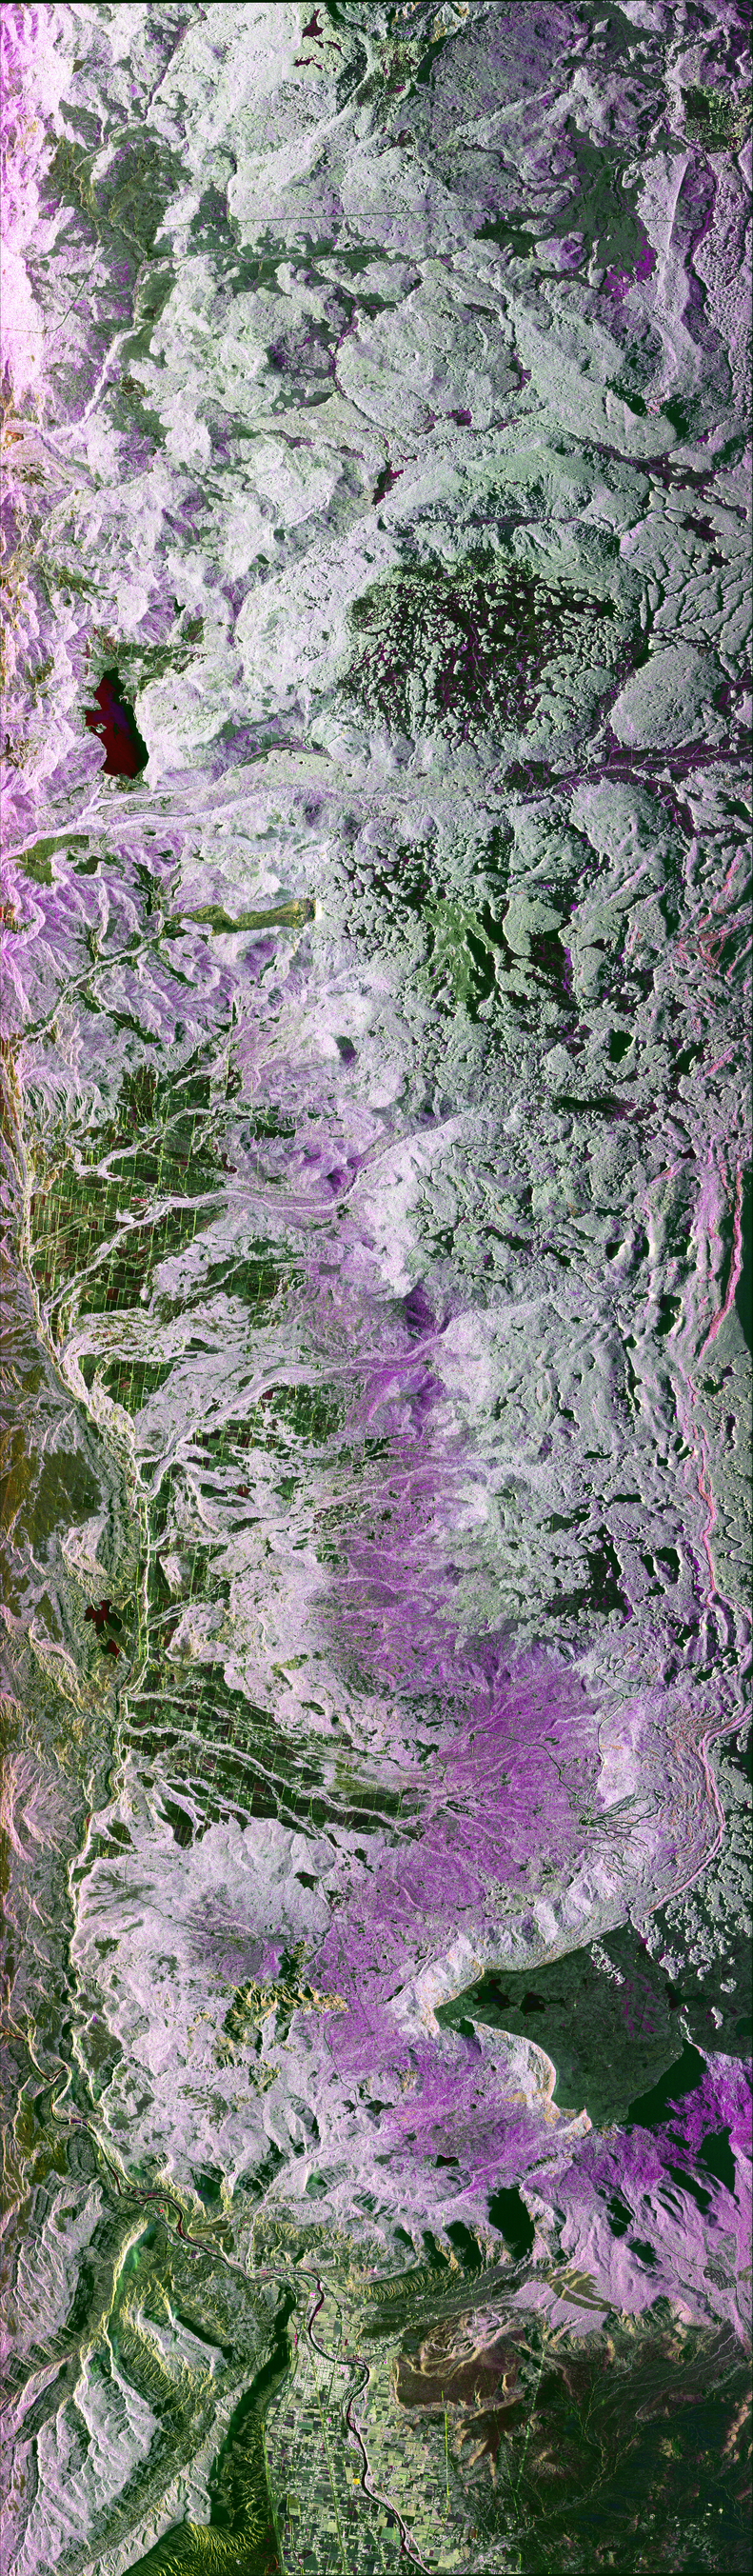
\includegraphics[width=.3\linewidth]{Pauli}}
	\subcaptionbox{Codificação de cores: $R=|K_{d}|^2; G=|K_{h}|^2; B=|K_{s}|^2$\label{fig:Krogager}}{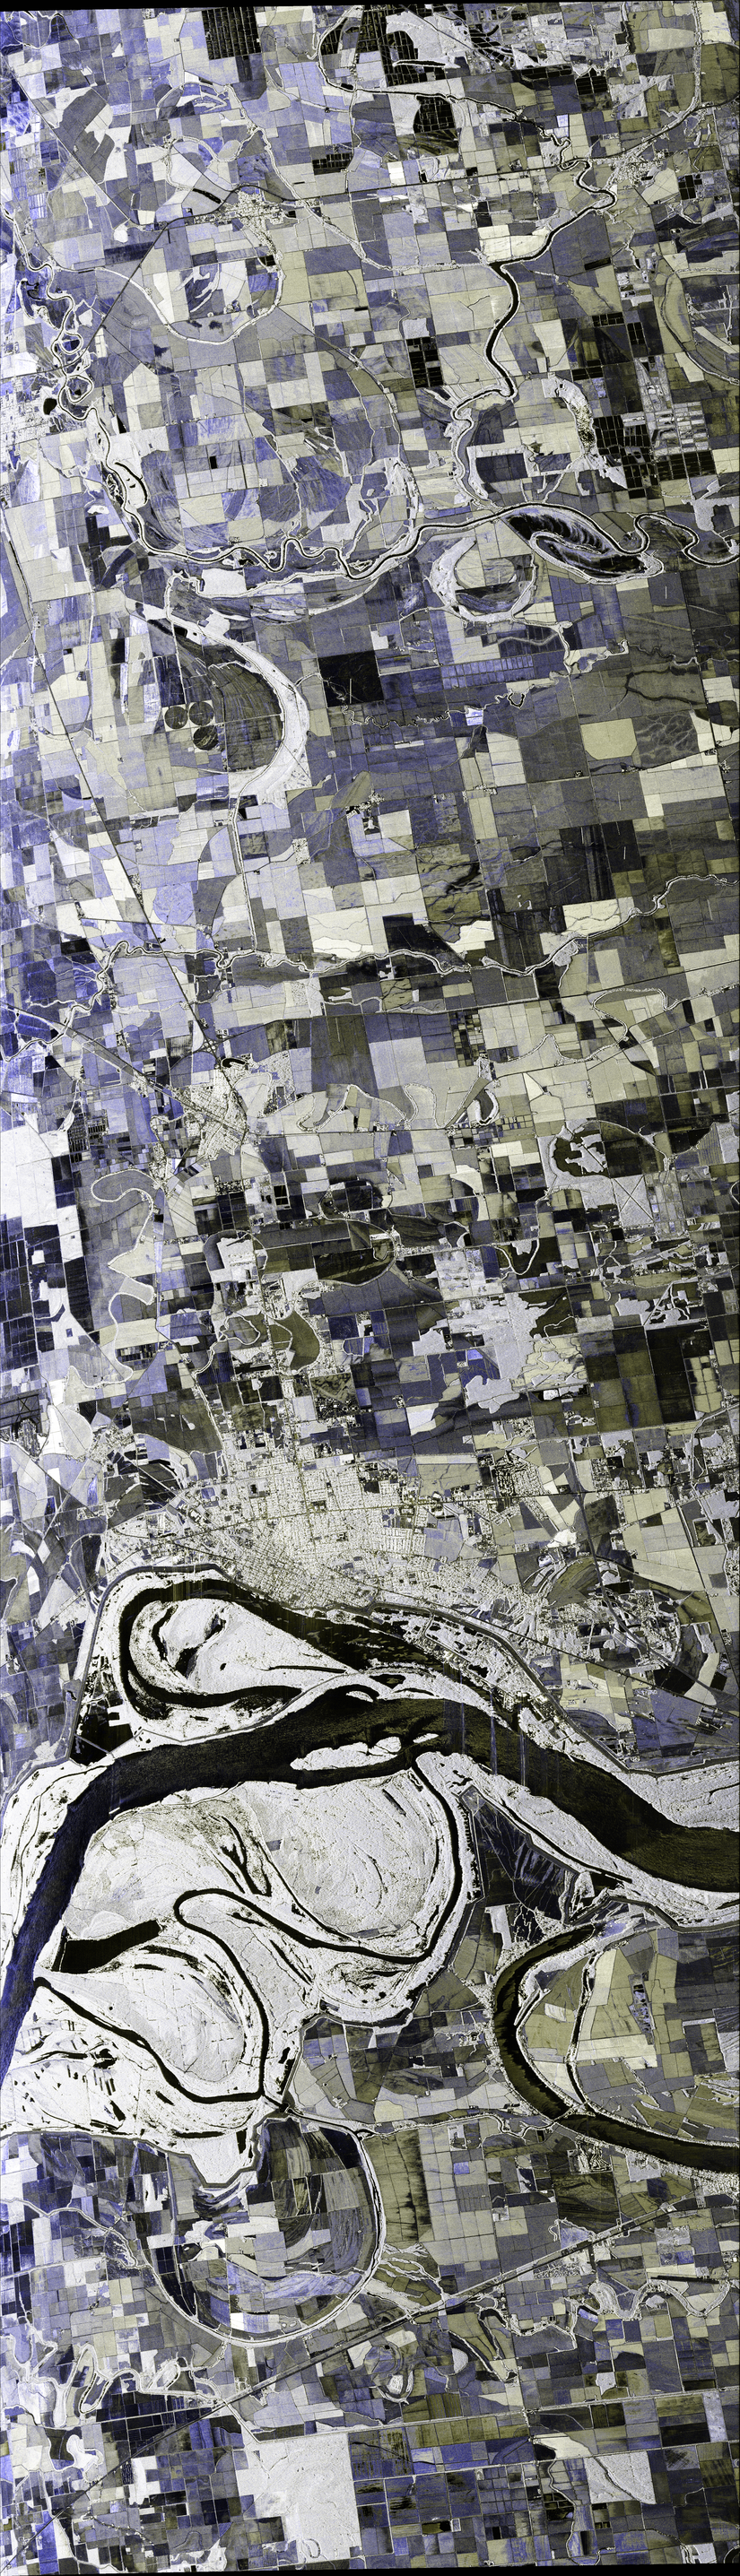
\includegraphics[width=.3\linewidth]{Krogager}}
	\subcaptionbox{Codificação de cores: $R=B_{0T}+B_{T}; G=B_{0T}+B_{T}; B=2A_{0}$
	\label{fig:Hyunen}}{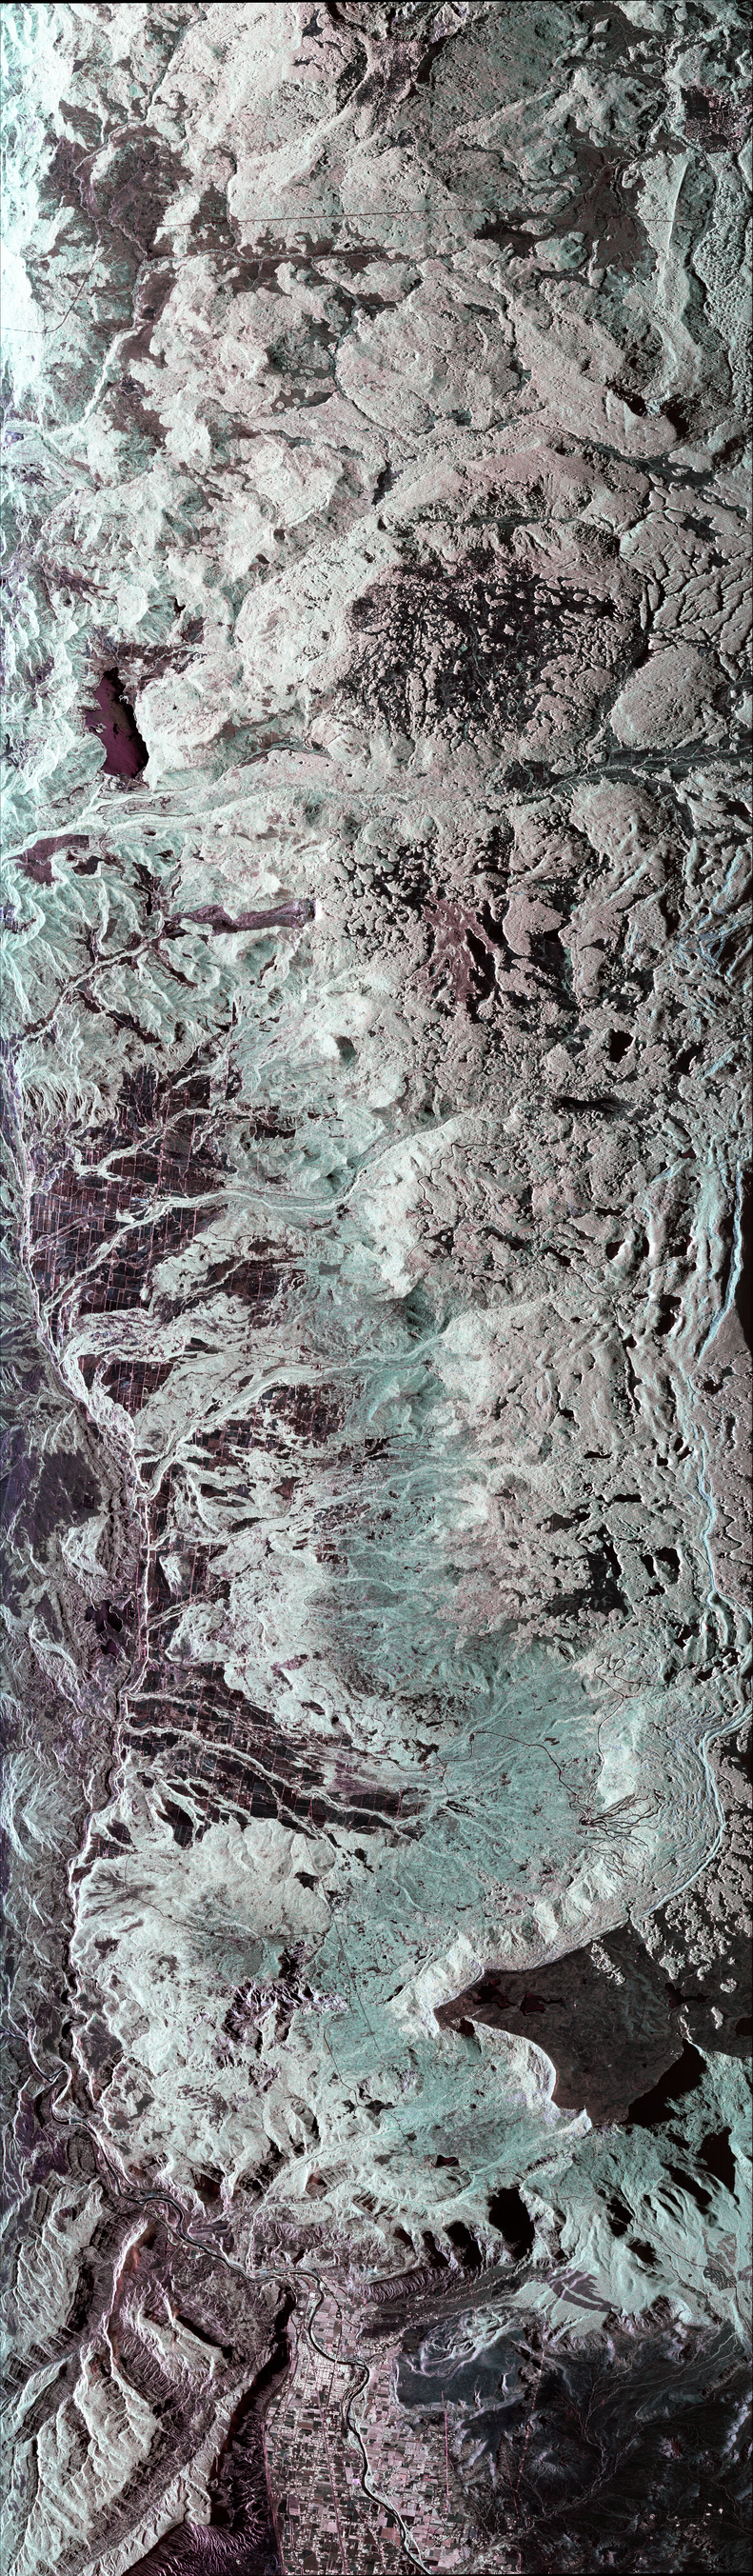
\includegraphics[width=.3\linewidth]{Hyunen}}
\caption{Visualização das decomposições}
\end{figure}

%=======================================================================================================================================================
\newpage
\section{CONCLUSÃO}

Apesar de grandes avanços registado na área de polarimetria de radar e um grande volume de dados disponibilizados à comunidade cientifica, o problema continua sendo nas ferramentas para interpretação desses dados. O presente relatório consiste em demostrar uma abordagem sobre sensoriamento remoto através de radar de abertura sintética SAR com auxílio das técnicas de polarimetria aplicadas ao processamento das imagens SAR. Isso serviu de base para modelagem dos algoritmo aplicados no desenvolvimento das funções para processamento, análise e visualização das imagens SAR.

As contribuições atuais: 

\begin{itemize}
    \item avaliação das outras técnicas da decomposições como:  CAMEROON, BARNES-HOLM, YANG, CLOUDE;
    \item prototipação de uma biblioteca que contém os algoritmos de visualização;
    \item disponibilidade da biblioteca para comunidade acadêmica em geral.  
\end{itemize}

\newpage
\bibliographystyle{unsrt}
\bibliography{ref}

\end{document}
    